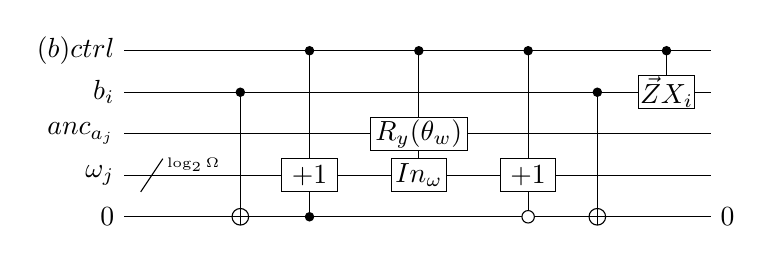
\begin{tikzpicture}[scale=1.000000,x=1pt,y=1pt]
\filldraw[color=white] (0.000000, -7.500000) rectangle (212.000000, 67.500000);
% Drawing wires
% Line 1: ctrl W \text{(b) }ctrl
\draw[color=black] (0.000000,60.000000) -- (212.000000,60.000000);
\draw[color=black] (0.000000,60.000000) node[left] {$\text{(b) }ctrl$};
% Line 2: i W b_i
\draw[color=black] (0.000000,45.000000) -- (212.000000,45.000000);
\draw[color=black] (0.000000,45.000000) node[left] {$b_i$};
% Line 3: anc_a W anc_{a_j}
\draw[color=black] (0.000000,30.000000) -- (212.000000,30.000000);
\draw[color=black] (0.000000,30.000000) node[left] {$anc_{a_j}$};
% Line 4: j W \omega_j
\draw[color=black] (0.000000,15.000000) -- (212.000000,15.000000);
\draw[color=black] (0.000000,15.000000) node[left] {$\omega_j$};
% Line 5: c0 W 0 0
\draw[color=black] (0.000000,0.000000) -- (212.000000,0.000000);
\draw[color=black] (0.000000,0.000000) node[left] {$0$};
% Done with wires; drawing gates
% Line 7: j / ^{\log_2{\Omega}}
\draw (6.000000, 9.000000) -- (14.000000, 21.000000);
\draw (12.000000, 18.000000) node[right] {$\scriptstyle{^{\log_2{\Omega}}}$};
% Line 8: ctrl i anc_a j c0 LABEL width=1
% Line 10: i +c0
\draw (42.000000,45.000000) -- (42.000000,0.000000);
\filldraw (42.000000, 45.000000) circle(1.500000pt);
\begin{scope}
\draw[fill=white] (42.000000, 0.000000) circle(3.000000pt);
\clip (42.000000, 0.000000) circle(3.000000pt);
\draw (39.000000, 0.000000) -- (45.000000, 0.000000);
\draw (42.000000, -3.000000) -- (42.000000, 3.000000);
\end{scope}
% Line 11: j G width=20 $+1$ ctrl c0
\draw (67.000000,60.000000) -- (67.000000,0.000000);
\begin{scope}
\draw[fill=white] (67.000000, 15.000000) +(-45.000000:14.142136pt and 8.485281pt) -- +(45.000000:14.142136pt and 8.485281pt) -- +(135.000000:14.142136pt and 8.485281pt) -- +(225.000000:14.142136pt and 8.485281pt) -- cycle;
\clip (67.000000, 15.000000) +(-45.000000:14.142136pt and 8.485281pt) -- +(45.000000:14.142136pt and 8.485281pt) -- +(135.000000:14.142136pt and 8.485281pt) -- +(225.000000:14.142136pt and 8.485281pt) -- cycle;
\draw (67.000000, 15.000000) node {$+1$};
\end{scope}
\filldraw (67.000000, 60.000000) circle(1.500000pt);
\filldraw (67.000000, 0.000000) circle(1.500000pt);
% Line 12: anc_a G:width=35 $R_y(\theta_w)$ j G:width=20 $In_\omega$ ctrl
\draw (106.500000,60.000000) -- (106.500000,15.000000);
\begin{scope}
\draw[fill=white] (106.500000, 30.000000) +(-45.000000:24.748737pt and 8.485281pt) -- +(45.000000:24.748737pt and 8.485281pt) -- +(135.000000:24.748737pt and 8.485281pt) -- +(225.000000:24.748737pt and 8.485281pt) -- cycle;
\clip (106.500000, 30.000000) +(-45.000000:24.748737pt and 8.485281pt) -- +(45.000000:24.748737pt and 8.485281pt) -- +(135.000000:24.748737pt and 8.485281pt) -- +(225.000000:24.748737pt and 8.485281pt) -- cycle;
\draw (106.500000, 30.000000) node {$R_y(\theta_w)$};
\end{scope}
\begin{scope}
\draw[fill=white] (106.500000, 15.000000) +(-45.000000:14.142136pt and 8.485281pt) -- +(45.000000:14.142136pt and 8.485281pt) -- +(135.000000:14.142136pt and 8.485281pt) -- +(225.000000:14.142136pt and 8.485281pt) -- cycle;
\clip (106.500000, 15.000000) +(-45.000000:14.142136pt and 8.485281pt) -- +(45.000000:14.142136pt and 8.485281pt) -- +(135.000000:14.142136pt and 8.485281pt) -- +(225.000000:14.142136pt and 8.485281pt) -- cycle;
\draw (106.500000, 15.000000) node {$In_\omega$};
\end{scope}
\filldraw (106.500000, 60.000000) circle(1.500000pt);
% Line 13: j G width=20 $+1$ ctrl -c0
\draw (146.000000,60.000000) -- (146.000000,0.000000);
\begin{scope}
\draw[fill=white] (146.000000, 15.000000) +(-45.000000:14.142136pt and 8.485281pt) -- +(45.000000:14.142136pt and 8.485281pt) -- +(135.000000:14.142136pt and 8.485281pt) -- +(225.000000:14.142136pt and 8.485281pt) -- cycle;
\clip (146.000000, 15.000000) +(-45.000000:14.142136pt and 8.485281pt) -- +(45.000000:14.142136pt and 8.485281pt) -- +(135.000000:14.142136pt and 8.485281pt) -- +(225.000000:14.142136pt and 8.485281pt) -- cycle;
\draw (146.000000, 15.000000) node {$+1$};
\end{scope}
\filldraw (146.000000, 60.000000) circle(1.500000pt);
\draw[fill=white] (146.000000, 0.000000) circle(2.250000pt);
% Line 14: i +c0
\draw (171.000000,45.000000) -- (171.000000,0.000000);
\filldraw (171.000000, 45.000000) circle(1.500000pt);
\begin{scope}
\draw[fill=white] (171.000000, 0.000000) circle(3.000000pt);
\clip (171.000000, 0.000000) circle(3.000000pt);
\draw (168.000000, 0.000000) -- (174.000000, 0.000000);
\draw (171.000000, -3.000000) -- (171.000000, 3.000000);
\end{scope}
% Line 16: i G width=20 $\vec{Z}X_i$ ctrl
\draw (196.000000,60.000000) -- (196.000000,45.000000);
\begin{scope}
\draw[fill=white] (196.000000, 45.000000) +(-45.000000:14.142136pt and 8.485281pt) -- +(45.000000:14.142136pt and 8.485281pt) -- +(135.000000:14.142136pt and 8.485281pt) -- +(225.000000:14.142136pt and 8.485281pt) -- cycle;
\clip (196.000000, 45.000000) +(-45.000000:14.142136pt and 8.485281pt) -- +(45.000000:14.142136pt and 8.485281pt) -- +(135.000000:14.142136pt and 8.485281pt) -- +(225.000000:14.142136pt and 8.485281pt) -- cycle;
\draw (196.000000, 45.000000) node {$\vec{Z}X_i$};
\end{scope}
\filldraw (196.000000, 60.000000) circle(1.500000pt);
% Done with gates; drawing ending labels
\draw[color=black] (212.000000,0.000000) node[right] {$0$};
% Done with ending labels; drawing cut lines and comments
% Done with comments
\end{tikzpicture}
